\documentclass[12pt, a4paper]{article}
\title{Спектральный анализ электрических сигналов (3.6.1)}
\author{Стеценко Георгий, Б02-312}
\date{}
% !TeX encoding = UTF-8

\usepackage{geometry}
\usepackage{amsmath, amsfonts, amssymb, amsthm} % стандартный набор AMS-пакетов для математ. текстов
\usepackage{mathtext}
\usepackage[utf8]{inputenc} % кодировка utf8
\usepackage[russian]{babel} % русский язык
\usepackage[pdftex,dvipsnames]{xcolor} % работа с цветами
\usepackage[pdftex]{graphicx} % графика (картинки)
\usepackage{tikz,pgfplots} % рисунки
\usepackage{indentfirst}
%\usepackage[labelfont=bf,labelsep=endash,skip=3pt]{caption} % подпись картинок
% \usepackage{fancyhdr,pageslts} % настройка колонтитулов
\usepackage{enumitem} % работа со списками
\usepackage{floatrow,multicol,multirow,longtable,hhline} % работа с таблицами
\usepackage{float,wrapfig} % плавающие объекты
\usepackage{tcolorbox} % рамка вокруг текста
%\usepackage[calc]{datetime2} % дата
\usepackage{bm} % жирное начертание в формулах
\usepackage{physics} % физический пакет
\DeclareMathAlphabet\mathbfcal{OMS}{cmsy}{b}{n}
\usepackage{pgfornament} % красивые рюшечки и вензеля
\usepackage{mdframed}
\usepackage{derivative}
\usepackage{mathrsfs} %EDS
\usepackage{soul} % strikethorugh
%\usepackage{boondox-cal}

% ----------------------------------------
% Настройка шрифта

% Просто закооментируйте следующую строчку, если не работает. Будет другой шрифт, правда :(
% \usepackage{pscyr}

% ----------------------------------------
% Стилевые настройки

\usepackage{boldline} % жирная линия после таблиц (чтобы не было ошибок, этот пакет должен подключаться именно тут!)
\floatsetup[table]{style=Plaintop,floatrowsep=qquad} % настройка оформления таблиц
\setlist[enumerate,itemize]{leftmargin=5mm,itemindent=10mm,itemsep=0mm,
listparindent=0em,labelsep=2mm,topsep=2mm,labelwidth=4mm} % настройки списков

\setlength{\columnsep}{0.5cm} % расстояние между колонками
\setlength{\parskip}{1pt} % расстояние до текста от колонтитула

%\usepackage{titlesec} % управление оформлением section
%\renewcommand{\thesection}{\Roman{section}}
%\titleformat{\section}[block]{\bfseries\large}{\thesection.}{5pt}{}

% ----------------------------------------
% Настройки полей
\geometry{
  left=10mm,
  top=10mm,
  right=10mm,
  bottom=15mm,
  marginparsep=0mm,
  marginparwidth=0mm,
  headheight=0pt,
  headsep=0pt,
footskip=20pt}

% ----------------------------------------
% Настройки колонтитулов и нумерации страниц
\pagenumbering{arabic}



\newcounter{ntask}
\setcounter{ntask}{0}


\newcommand{\arsh}{\mathrm{arsh} \,\,}
\newcommand{\arch}{\mathrm{arch} \,\,}
\newcommand{\arth}{\mathrm{arth} \,\,}
\newcommand{\arcth}{\mathrm{arcth} \,\,}
\renewcommand{\Re}{\operatorname{Re} \,}
\newcommand{\EDS}{\mathscr{E}}
\newcommand{\diffract}[1]{\frac{\mathrm{d}#1}{\mathrm{d}t}}

\newcommand{\kHz}{~\mathrm{kHz}}
\newcommand{\us}{~\mathrm{\mu s}}
\addto\captionsrussian{\def\refname{Источники}}

\begin{document}
\maketitle

\section{Цель работы}
Изучение спектрального состава периодических электрических сигналов.



\section{Теоретические сведения}
Ряд Фурье и спектральный анализ. Согласно теореме Фурье, любая периодическая функция может быть представлена в виде ряда (конечного или бесконечного) гармонических функций с разными частотами:

\begin{equation}
  f(t) = A_0/2 + \sum_{n=1}^{\infty} A_n \cos{(2\pi \nu_n t)} + B_n \sin{(2\pi \nu_n t)}
  \label{nophase}
\end{equation}

Коэффициенты разложения ($A_n$, $B_n$) можно найти как:
\begin{equation}
  A_n = \frac{2}{T} \int _0 ^ T f(t) \cdot \cos {(2\pi \nu_n t)}\,\mathrm{d}t,\quad B_n = \frac{2}{T} \int _0 ^ T f(t) \cdot \sin {(2\pi \nu_n t)}\,\mathrm{d}t
\end{equation}

Более удобно представление (\ref{nophase}) можно переписать как:
\begin{equation}
  f(t) = a_0/2 + \sum _ {n=1}^{\infty} a_n \cos{(2\pi \nu_n t + \varphi_n)}
\end{equation}

Кроме того, есть достаточно простая взаимосвязь между сигналом и его спектром. Если в сигнале встречается некоторое характерное время $\Delta t$, то в спектре встретится характерный масштаб ${\Delta \nu}$. При этом выполнено т.н. соотношение неопределённостей:
\begin{equation}
  \Delta \nu \cdot \Delta t \sim 1
  \label{ndef}
\end{equation}

Для последовательности прямоугольных импульсов длиной $\tau$ с периодом $T$ также известны коэффициенты разложения:
\begin{equation}
  a_n = \frac{2 \tau}{T} \frac{\sin {\pi n \tau /T}}{\pi n \tau /T}
  \label{rect_spectra}
\end{equation}

Для амплитудно-модудированного синусоидального сигнала $f(t) = A\cdot \cos (\omega t) \cdot (1+\eta\cdot \cos(\Omega t))$ просто находится спектр в следующем виде:
\begin{equation}
  f(t) = a_0 \cos \omega_0 t + \frac{\eta a_0}{2} \cos{(\omega_0 + \Omega)t} + \frac{\eta a0}{2} \cos{(\omega_0 - \Omega)t}
\end{equation}
\section{Методика измерений и результаты}
\textbf{В работе используются:} анализатор спектра (цифро­вой), генератор прямоугольных импульсов и сигналов специальной формы, осциллограф.

\subsection{Часть A. Прямоугольные импульсы.}
Подадим на осциллограф прямоугольные импульсы. Показания спектров прямоугольных импульсов приведены на рисунке \ref{a4spectra}.

\begin{figure}[H]
  \centering
  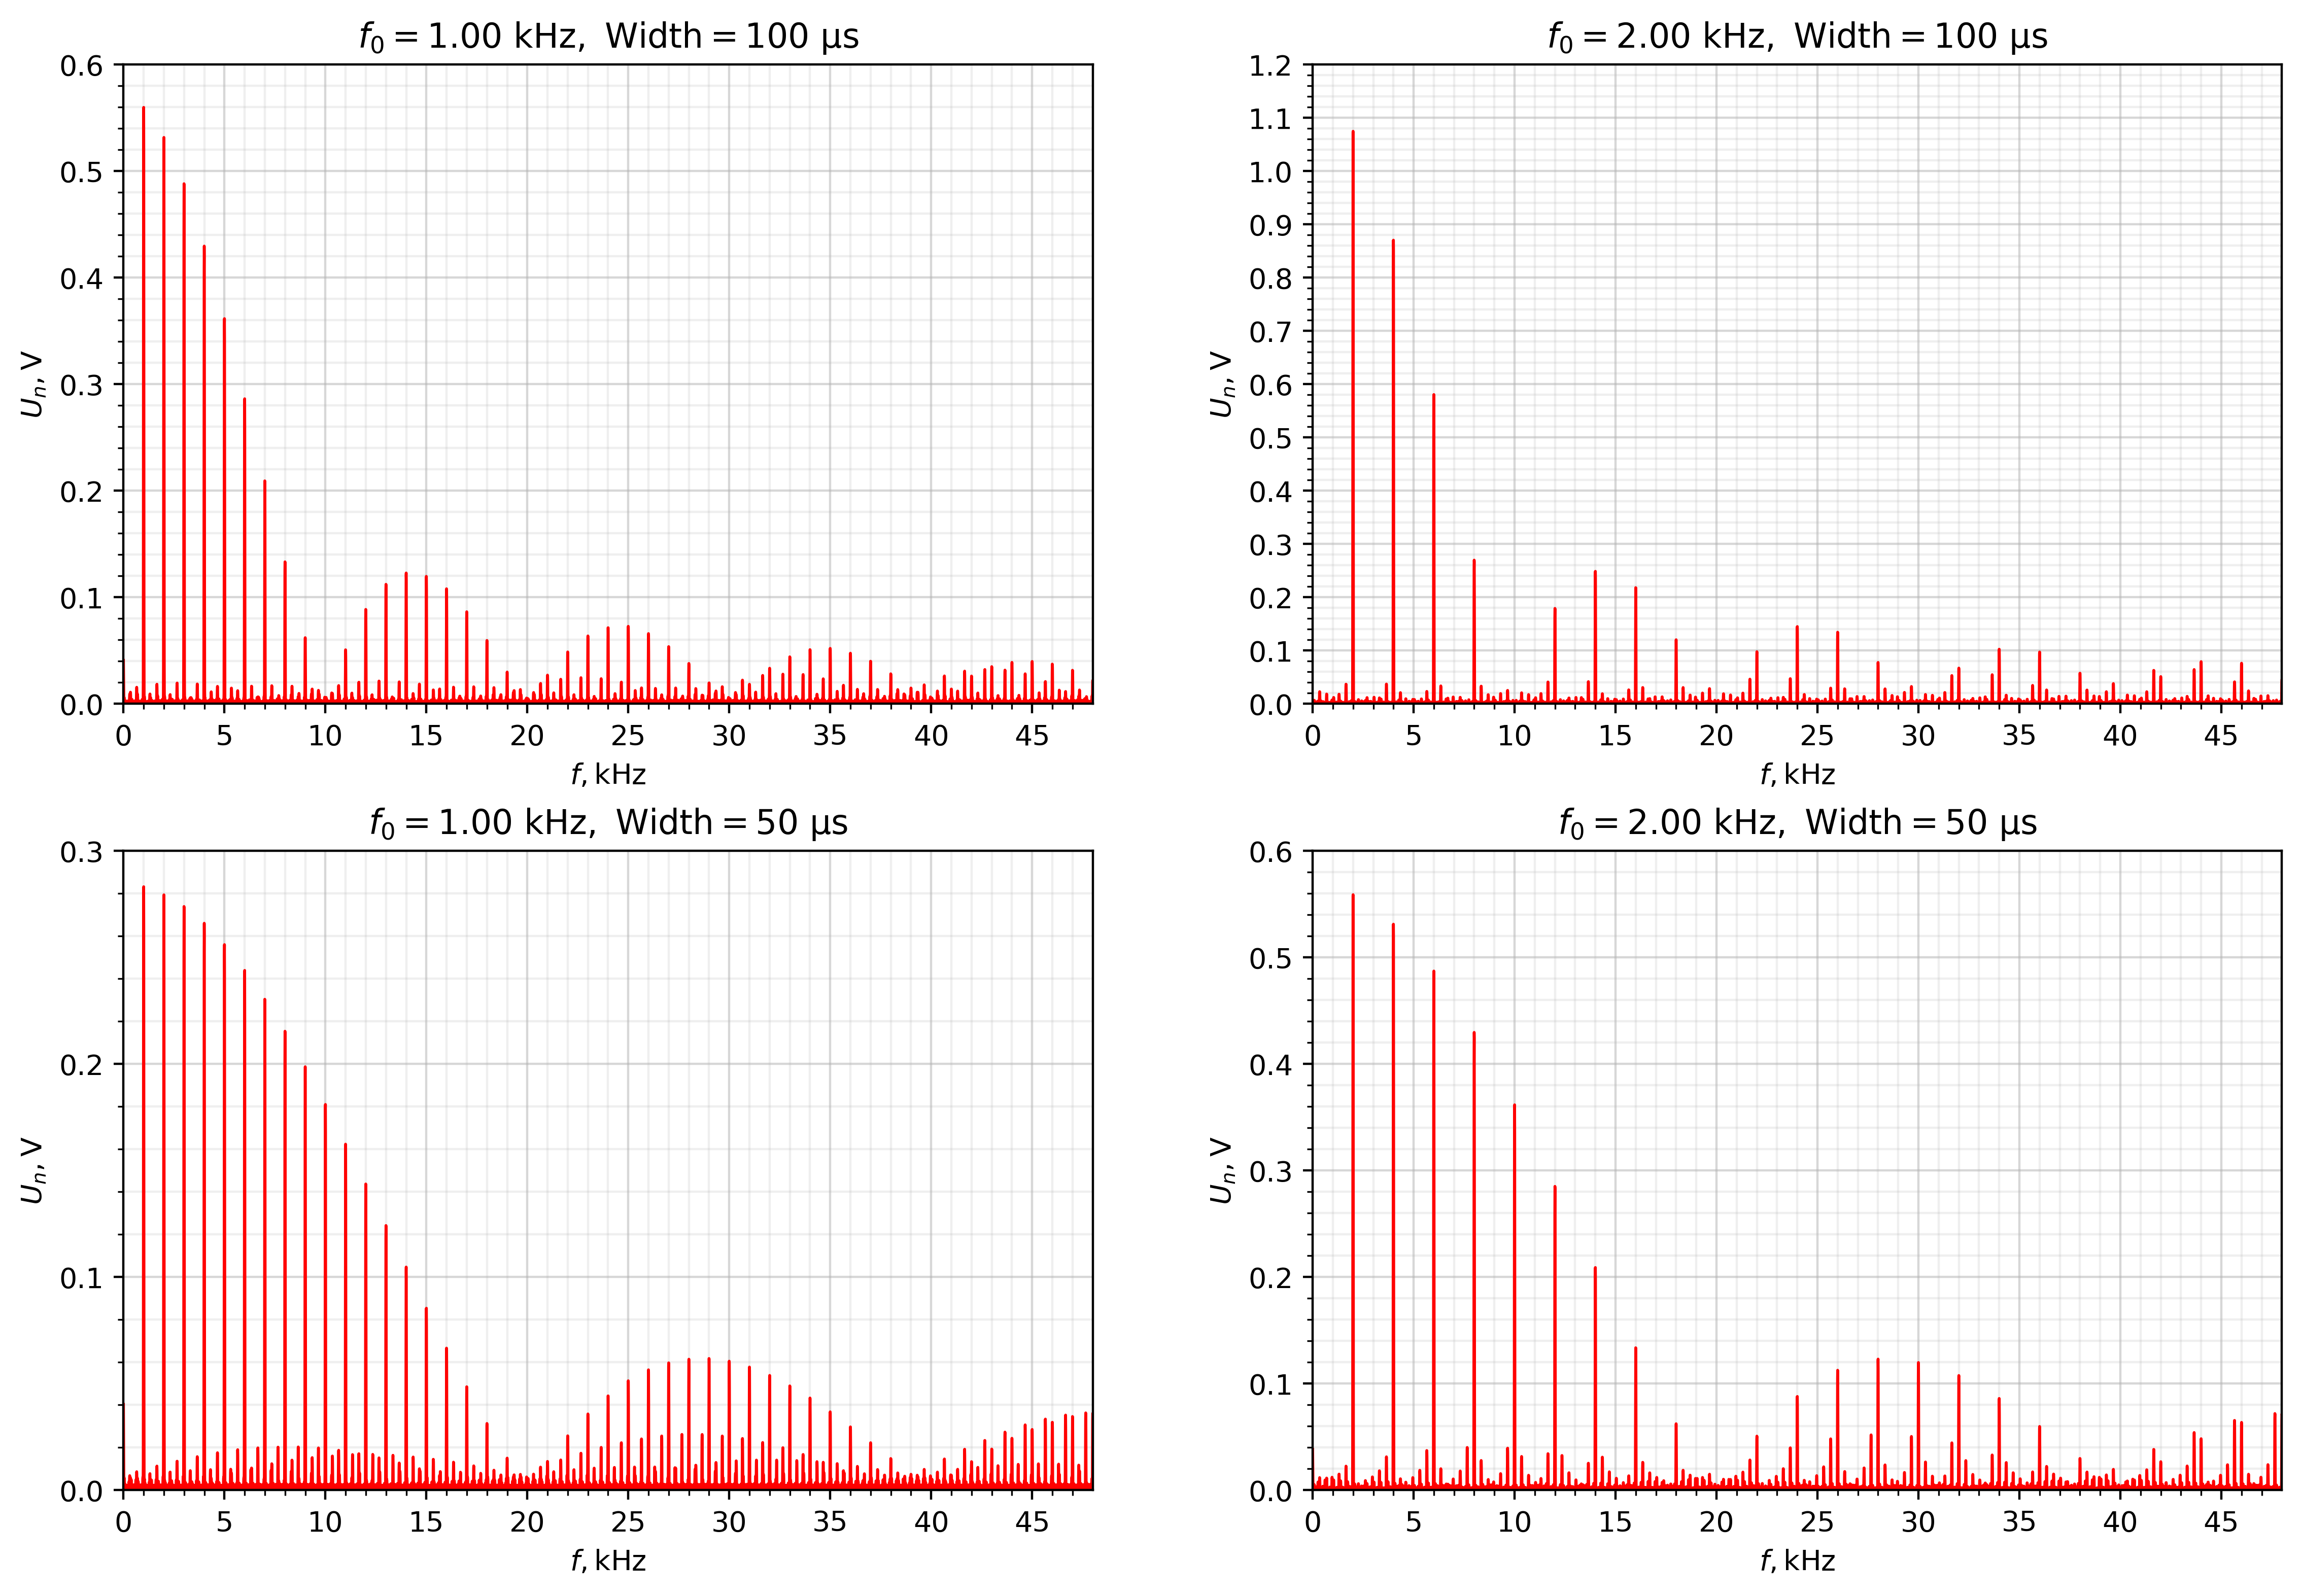
\includegraphics[width = 0.8\linewidth]{pics/A_4spectra}
  \caption{Спектры при различных параметрах прямоугольного сигнала}
  \label{a4spectra}
\end{figure}
По спектрам видно, что уменьшение ширины прямоугольного импульса (\textit{duty}) при неизменной частоте их подачи приводит к увеличению полной ширины спектра в соответсвующее число раз. При этом увеличение частоты подачи импульсов (обратного времени между началами ближайших импульсов) приводит к увеличению расстояния между ближайшими пиками в соответсвующее число раз.

Проведем сравнение экспериментального спектра (таблица \ref{spectracomparison}) с параметрами $2.00~\mathrm{kHz},~100~\mathrm{\mu s}$ с теоретическим (см. (\ref{rect_spectra})).

\begin{table}[H]
  \begin{tabular}{|l|l|l|l|l|l|l|l|}
    \hline
    n                            & 1     & 2     & 3     & 4     & 5     & 6     & 7     \\ \hline
    $\nu_n^\text{exp},~\mathrm{Hz}$   & 2.00  & 4.00  & 6.00  & 8.00  & --    & 12.00 & 14.00 \\ \hline
    $\nu_n^\text{th},~\mathrm{Hz}$    & 2.00  & 4.00  & 6.00  & 8.00  & 10.00 & 12.00 & 14.00 \\ \hline
    $|a_n|^\text{exp},~\mathrm{a.u.}$ & 1.074 & 0.870 & 0.580 & 0.269 & 0.000 & 0.179 & 0.248 \\ \hline
    $|a_n/a_1|^\text{exp}$            & 1.000 & 0.810 & 0.540 & 0.250 & 0.000 & 0.167 & 0.231 \\ \hline
    $|a_n/a_1|^\text{th}$             & 1.000 & 0.809 & 0.539 & 0.250 & 0.000 & 0.167 & 0.231 \\ \hline
  \end{tabular}
  \caption{Сравнение теоретического и экспериментального спектров.}
  \label{spectracomparison}
\end{table}

Теперь будем поочередно менять период $T$ и ширину сигнала $\tau$ и смотреть на изменение расстояния между гармониками $\delta \nu$ и полной ширины спектра $\Delta \nu$ соответственно.

\begin{table}[H]
  \begin{tabular}{|l|l|l|l|l|l|l|l|}
    \hline
    $T,~\mathrm{\mu s}$        & 100   & 200  & 500  & 1000 & 2000 & 2500 & \multirow{3}{*}{$\tau = 50~\mathrm{\mu s}$} \\ \cline{1-7}
    $1/T,~\mathrm{kHz}$        & 10.00 & 5.00 & 2.00 & 1.00 & 0.50 & 0.40 &                                             \\ \cline{1-7}
    $\delta \nu,~\mathrm{kHz}$ & 10.00 & 5.00 & 2.00 & 1.00 & 0.50 & 0.40 &                                             \\ \hline
    $\tau,~\mathrm{\mu s}$     & 50    & 60   & 70   & 80   & 90   & 100  & \multirow{3}{*}{$T = 1000~\mathrm{\mu s}$}  \\ \cline{1-7}
    $1/\tau,~\mathrm{kHz}$    & 20.0  & 16.7 & 14.3 & 12.5 & 11.1 & 10.0 &                                             \\ \cline{1-7}
    $\Delta \nu,~\mathrm{kHz}$ & 20.0  & 16.7 & 14.1 & 12.4 & 11.2 & 10.0 &                                             \\ \hline
  \end{tabular}
  \caption{Результаты измерений для проверки соотношений неопредёленности}
  \label{ndeftable}
\end{table}

Так как $\tau$ и $T$ могут быть не кратными друг другу, полная ширина спектра $\Delta \nu$ искалась экстраполяцией пиков, близких к корню их огибающей.

Характерная погрешность измерения не превышает погрешность, обусловленную дискретизацией ($<2\%$ для любой из приведённых точек). Использование метода рядов (например, определение $\delta \nu$ по пикам под номерами $n$ и $n+m$) делает эту погрешность ещё меньше, и грубо её можно оценить сверху как $1\%$.

Можно было бы построить графики по результатам из таблицы \ref{ndeftable}, но это не требуется: в данном случае по данным отлично видно, что в большинстве случаев проверяемые величины совпадают вплоть до значащей цифры включительно. То есть соотношения неопредённостей (соотв. (\ref{ndef}) для $(T, \delta \nu)$, $(t, \Delta \nu)$) в пределах погрешности выполняются со знаком <<=>>:
$$T\cdot \delta \nu = 1, \quad t \cdot \Delta \nu = 1$$

\subsection{Часть B. Наблюдение спектра периодической последовательности цугов}
\begin{wrapfigure}[3]{r}{4.5cm}\vspace{-12mm}
  \centering
  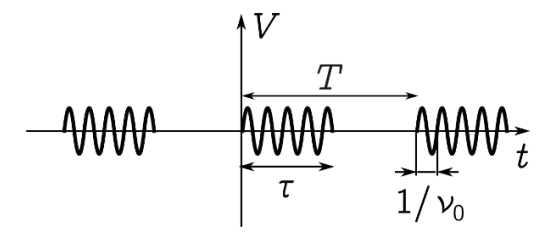
\includegraphics[width=4cm]{pics/zug}
  \caption{Форма цуга}
  \label{zug}
\end{wrapfigure}
Установим на источник режим подачи периодических импульсов синусоидальной формы (\textit{цугов}) (рис. \ref{zug}) с частотой несущей $f_0 = 50~\mathrm{kHz}$, периодом повторения $T = 1~\mathrm{ms}$, длительностью импульса $\tau = 100~\mathrm{\mu s}$.

\vspace{3mm}
\begin{figure}[H]
  \centering
  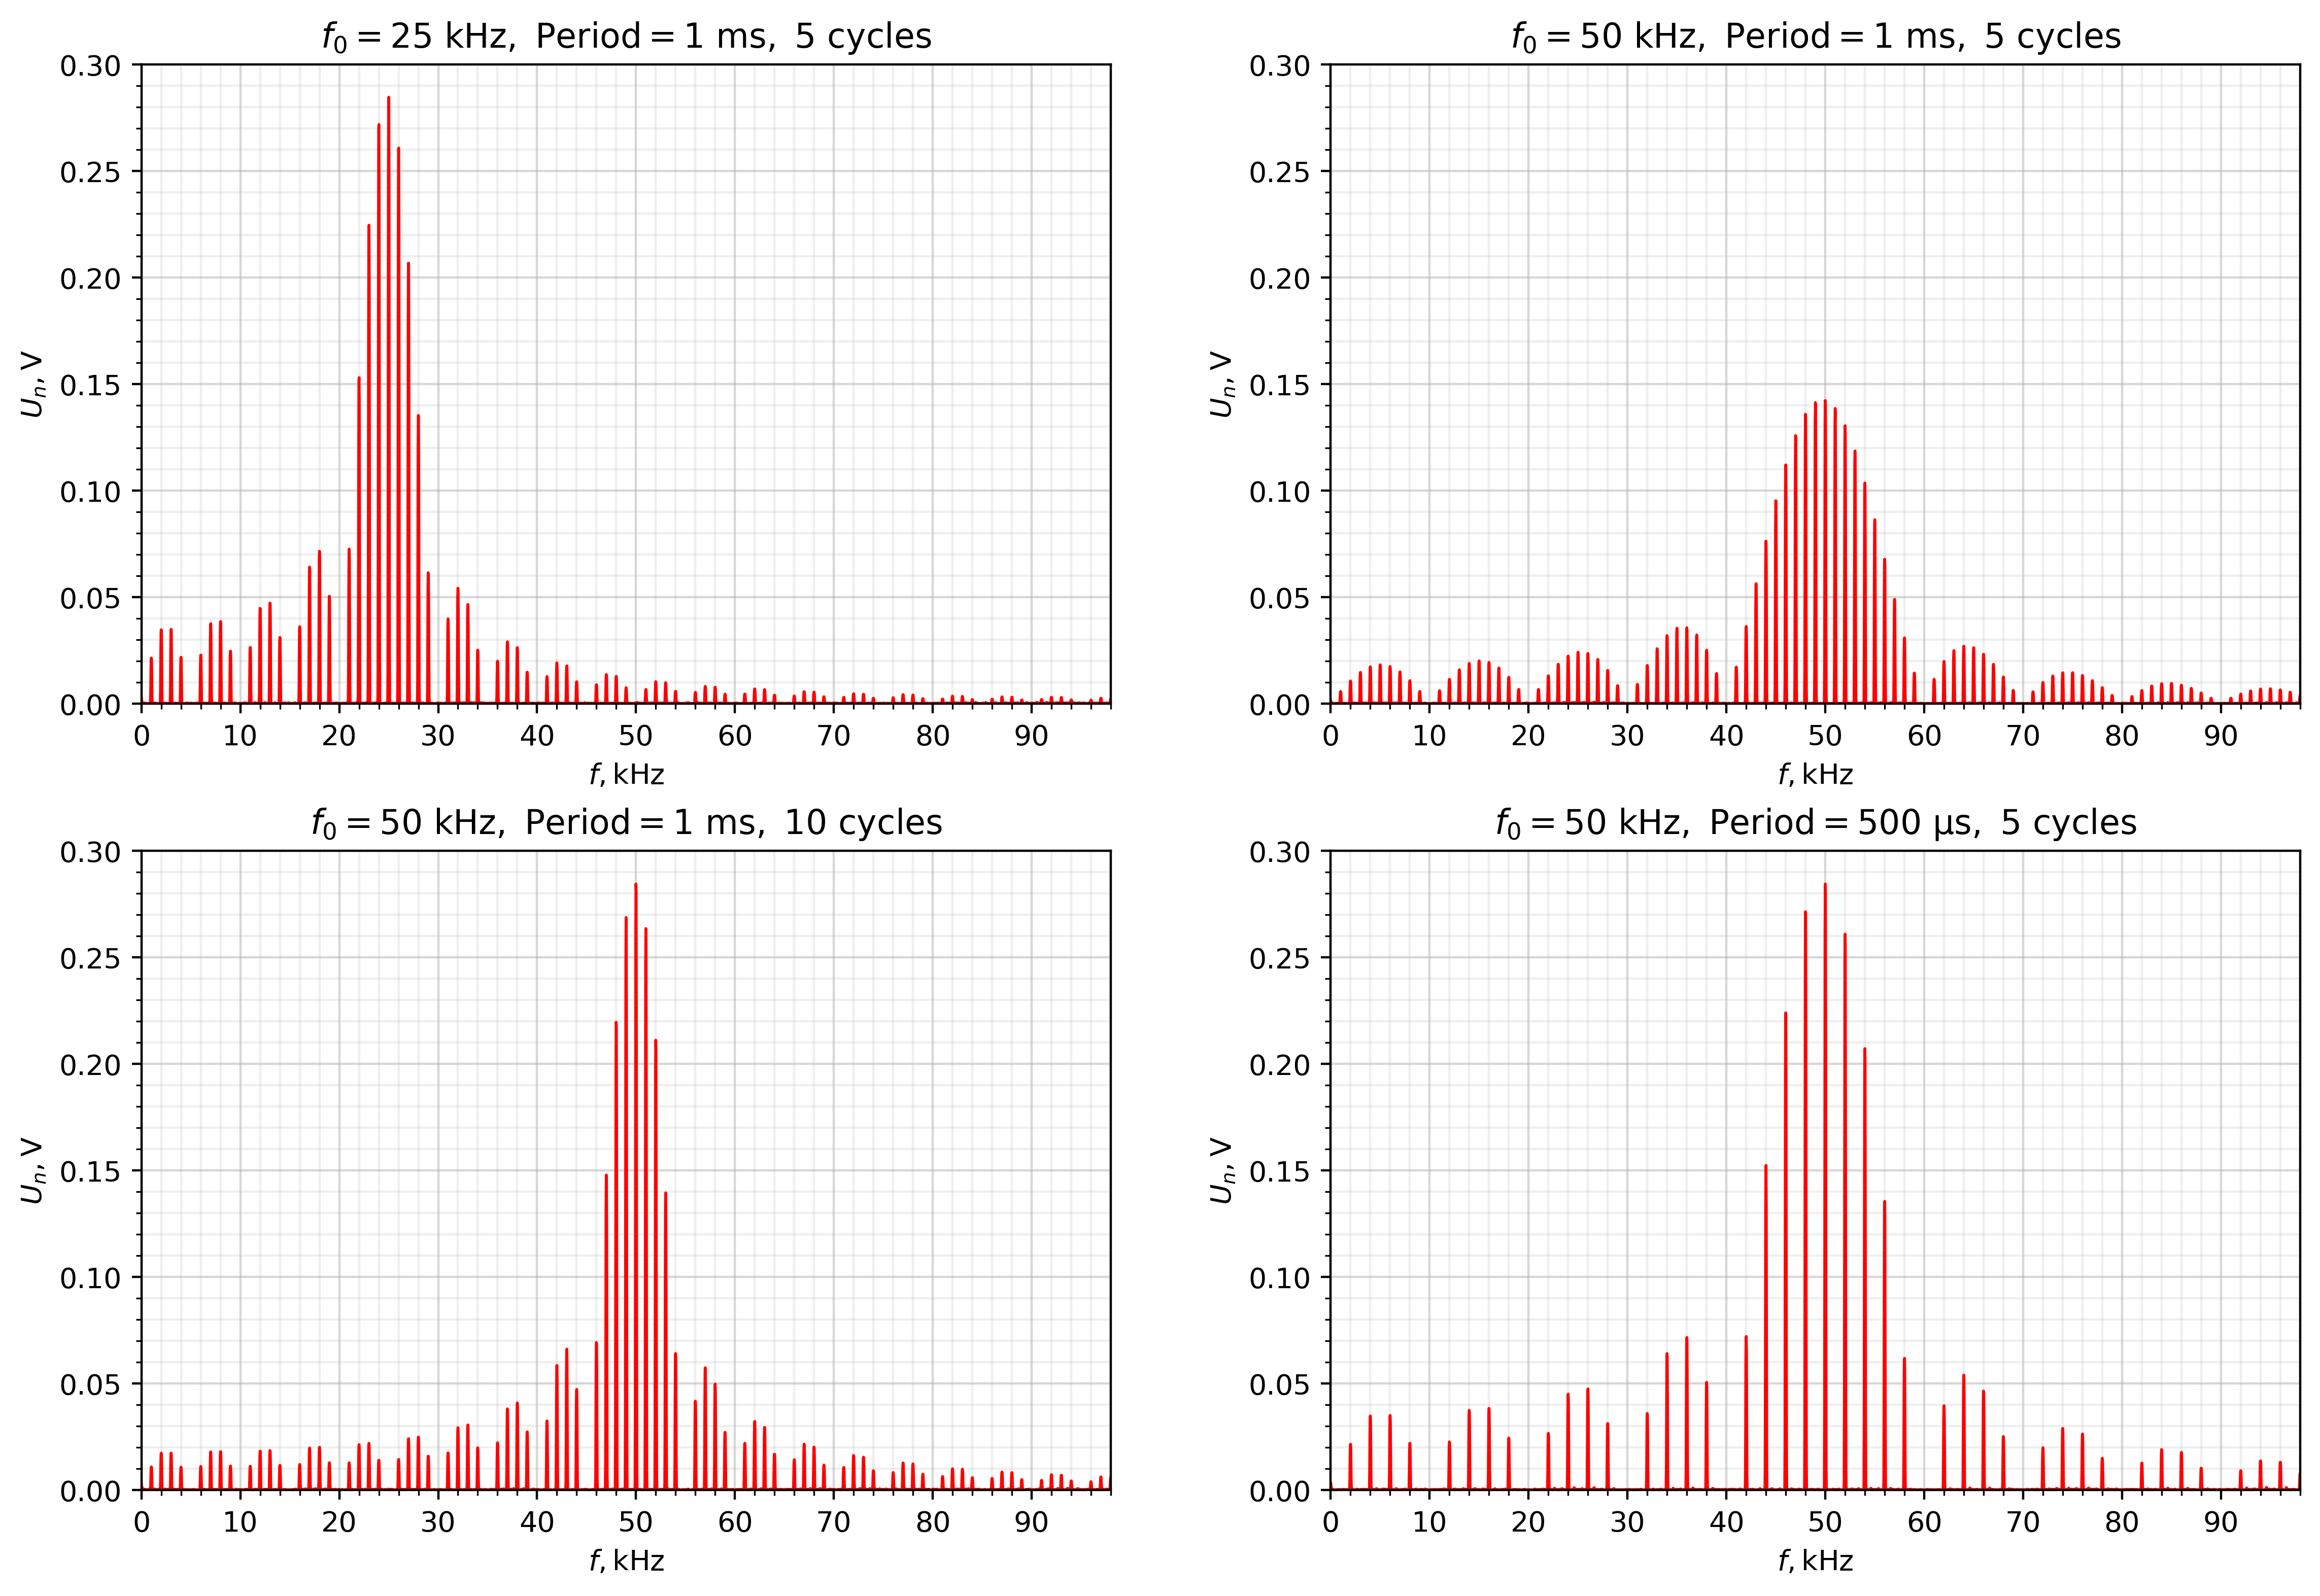
\includegraphics[width = 0.8\linewidth]{pics/B_4spectra}
  \caption{Спектры при различных параметрах цугов}
  \label{b4spectra}
\end{figure}

Видно, что соотношения неопределённостей выполнены (причём со знаком <<=>>): ширина спектра $\Delta f = f_0 / N$, расстояние между пиками $\delta f = \dfrac{1}{T}$.

\subsection{Часть D. Исследование спектра амплитудно-модулированного сигнала}
Установим на источнике режим модулированной синусоиды с несущей частотой $f_0 = 50\kHz$, частотой модуляции $f_m = 2\kHz$, глубиной модуляции $\eta = 50\%$. Полученный спектр изображён на рис. \ref{am}.

\begin{figure}[H]
  \centering
  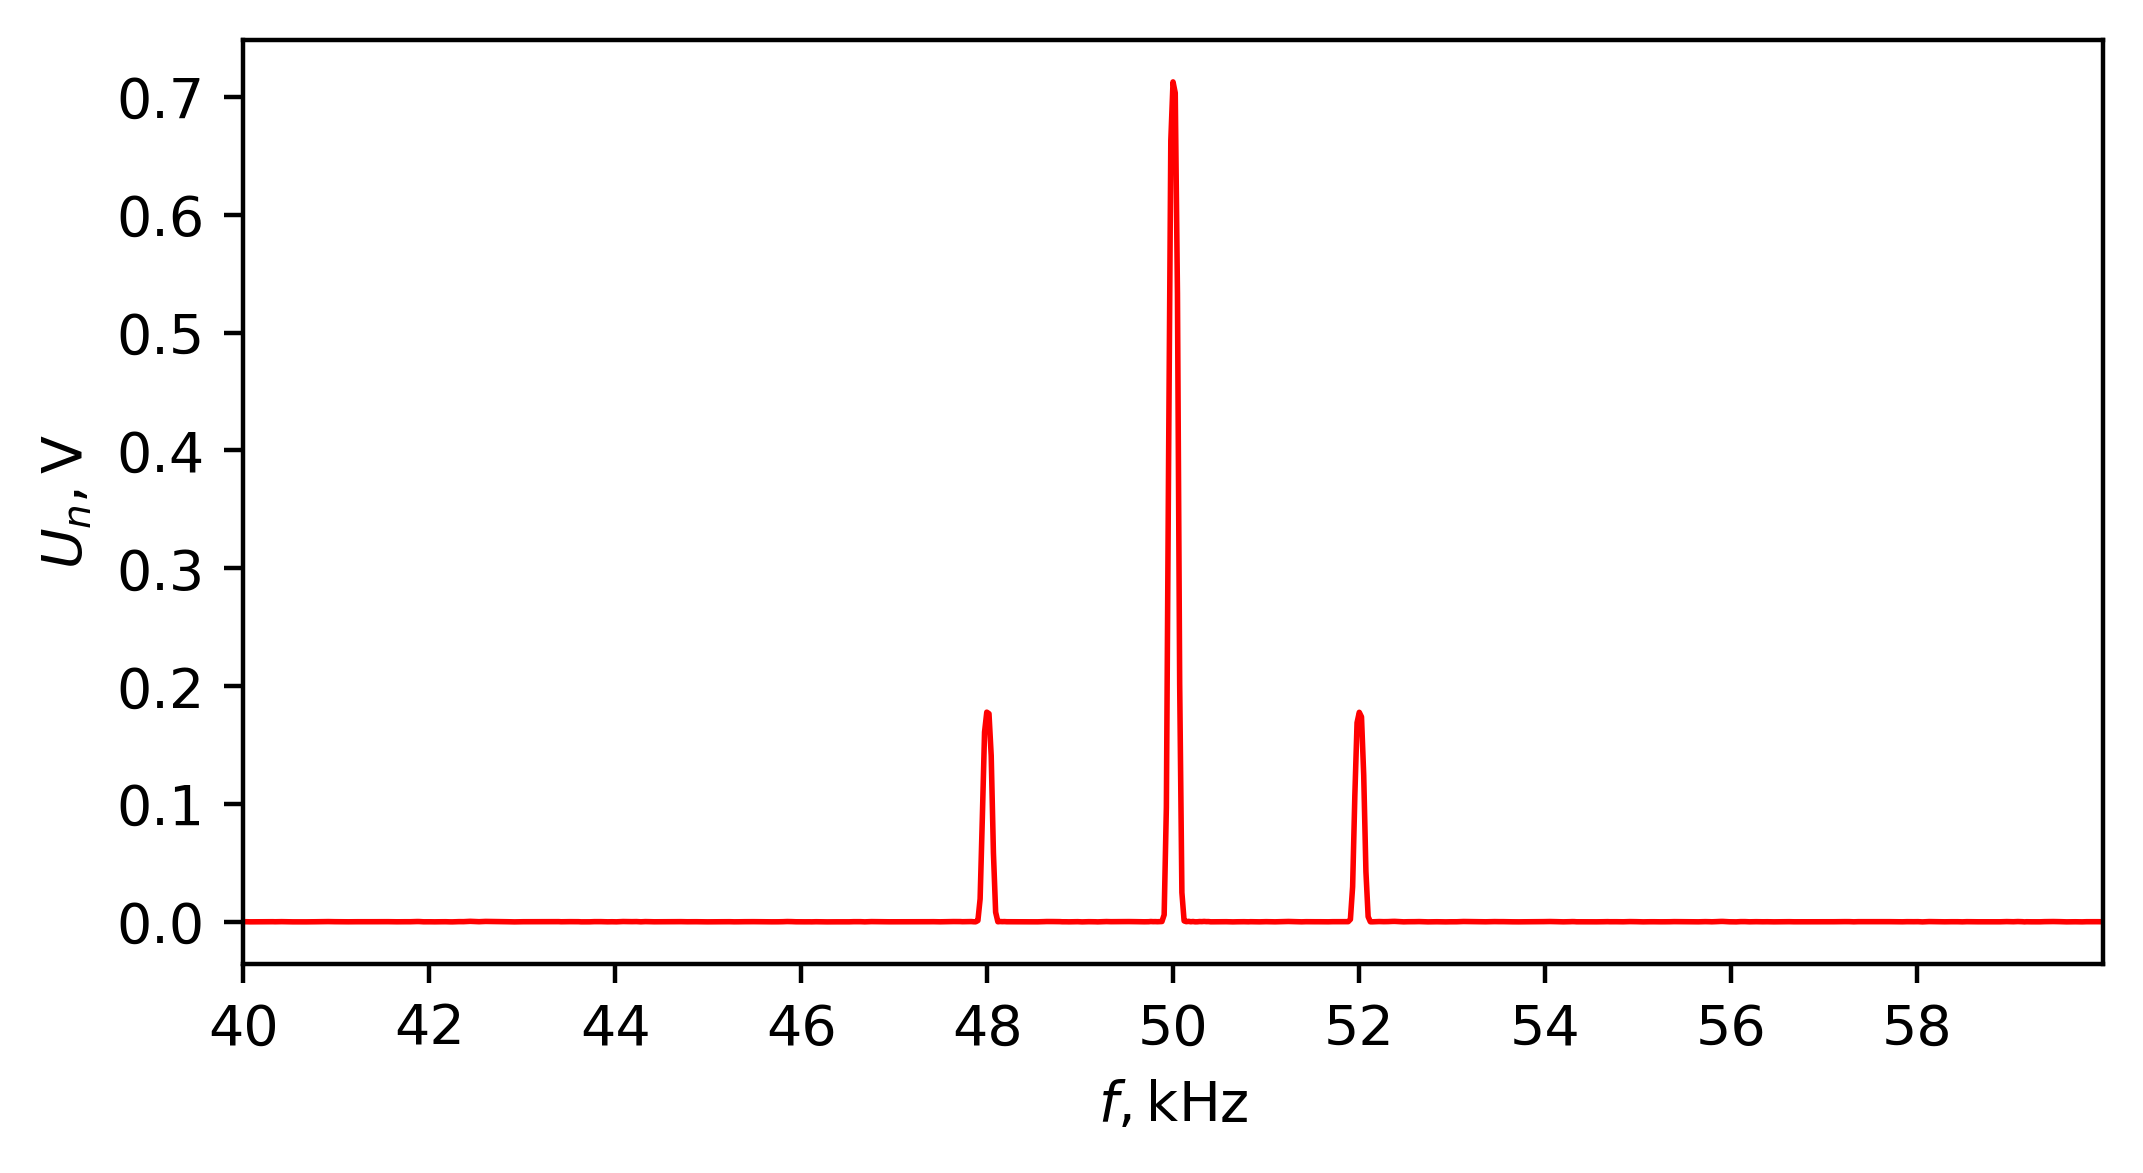
\includegraphics[width = 0.8\linewidth]{pics/am}
  \caption{Спектр амплитудно-модулированного сигнала}
  \label{am}
\end{figure}

\begin{table}[h!]
  \centering
  \begin{tabular}{|c|c|c|c|c|c|c|c|c|c|c|}
    \hline m, \% & 10 & 20& 30& 40& 50& 60& 70 & 80 &90 &100\\ \hline
    $a_{side}$, mV & 28.1 & 64.6& 106.7   &142.6& 177.9& 213.6& 249.5& 285.1&320.9&356.8\\ \hline
    $a_0,~\mathrm{mV}$ & 712.8 & 712.7& 712.8& 712.7& 712.7& 712.5& 712.2& 712.2&712.2&709.3\\ \hline
    $(a_{side}/a_0)^\text{exp}$ & 0.039& 0.091& 0.150& 0.200& 0.250& 0.300& 0.350& 0.400&0.451&0.503\\ \hline
    $(a_{side}/a_0)^\text{th}$ & 0.050 & 0.100 & 0.150 & 0.200 & 0.250 & 0.300 & 0.350 & 0.400 & 0.450 & 0.500 \\ \hline
  \end{tabular}
  \label{amdata}
\end{table}

По полученным данным построим график \ref{amplot}:
\begin{figure}[H]
  \centering
  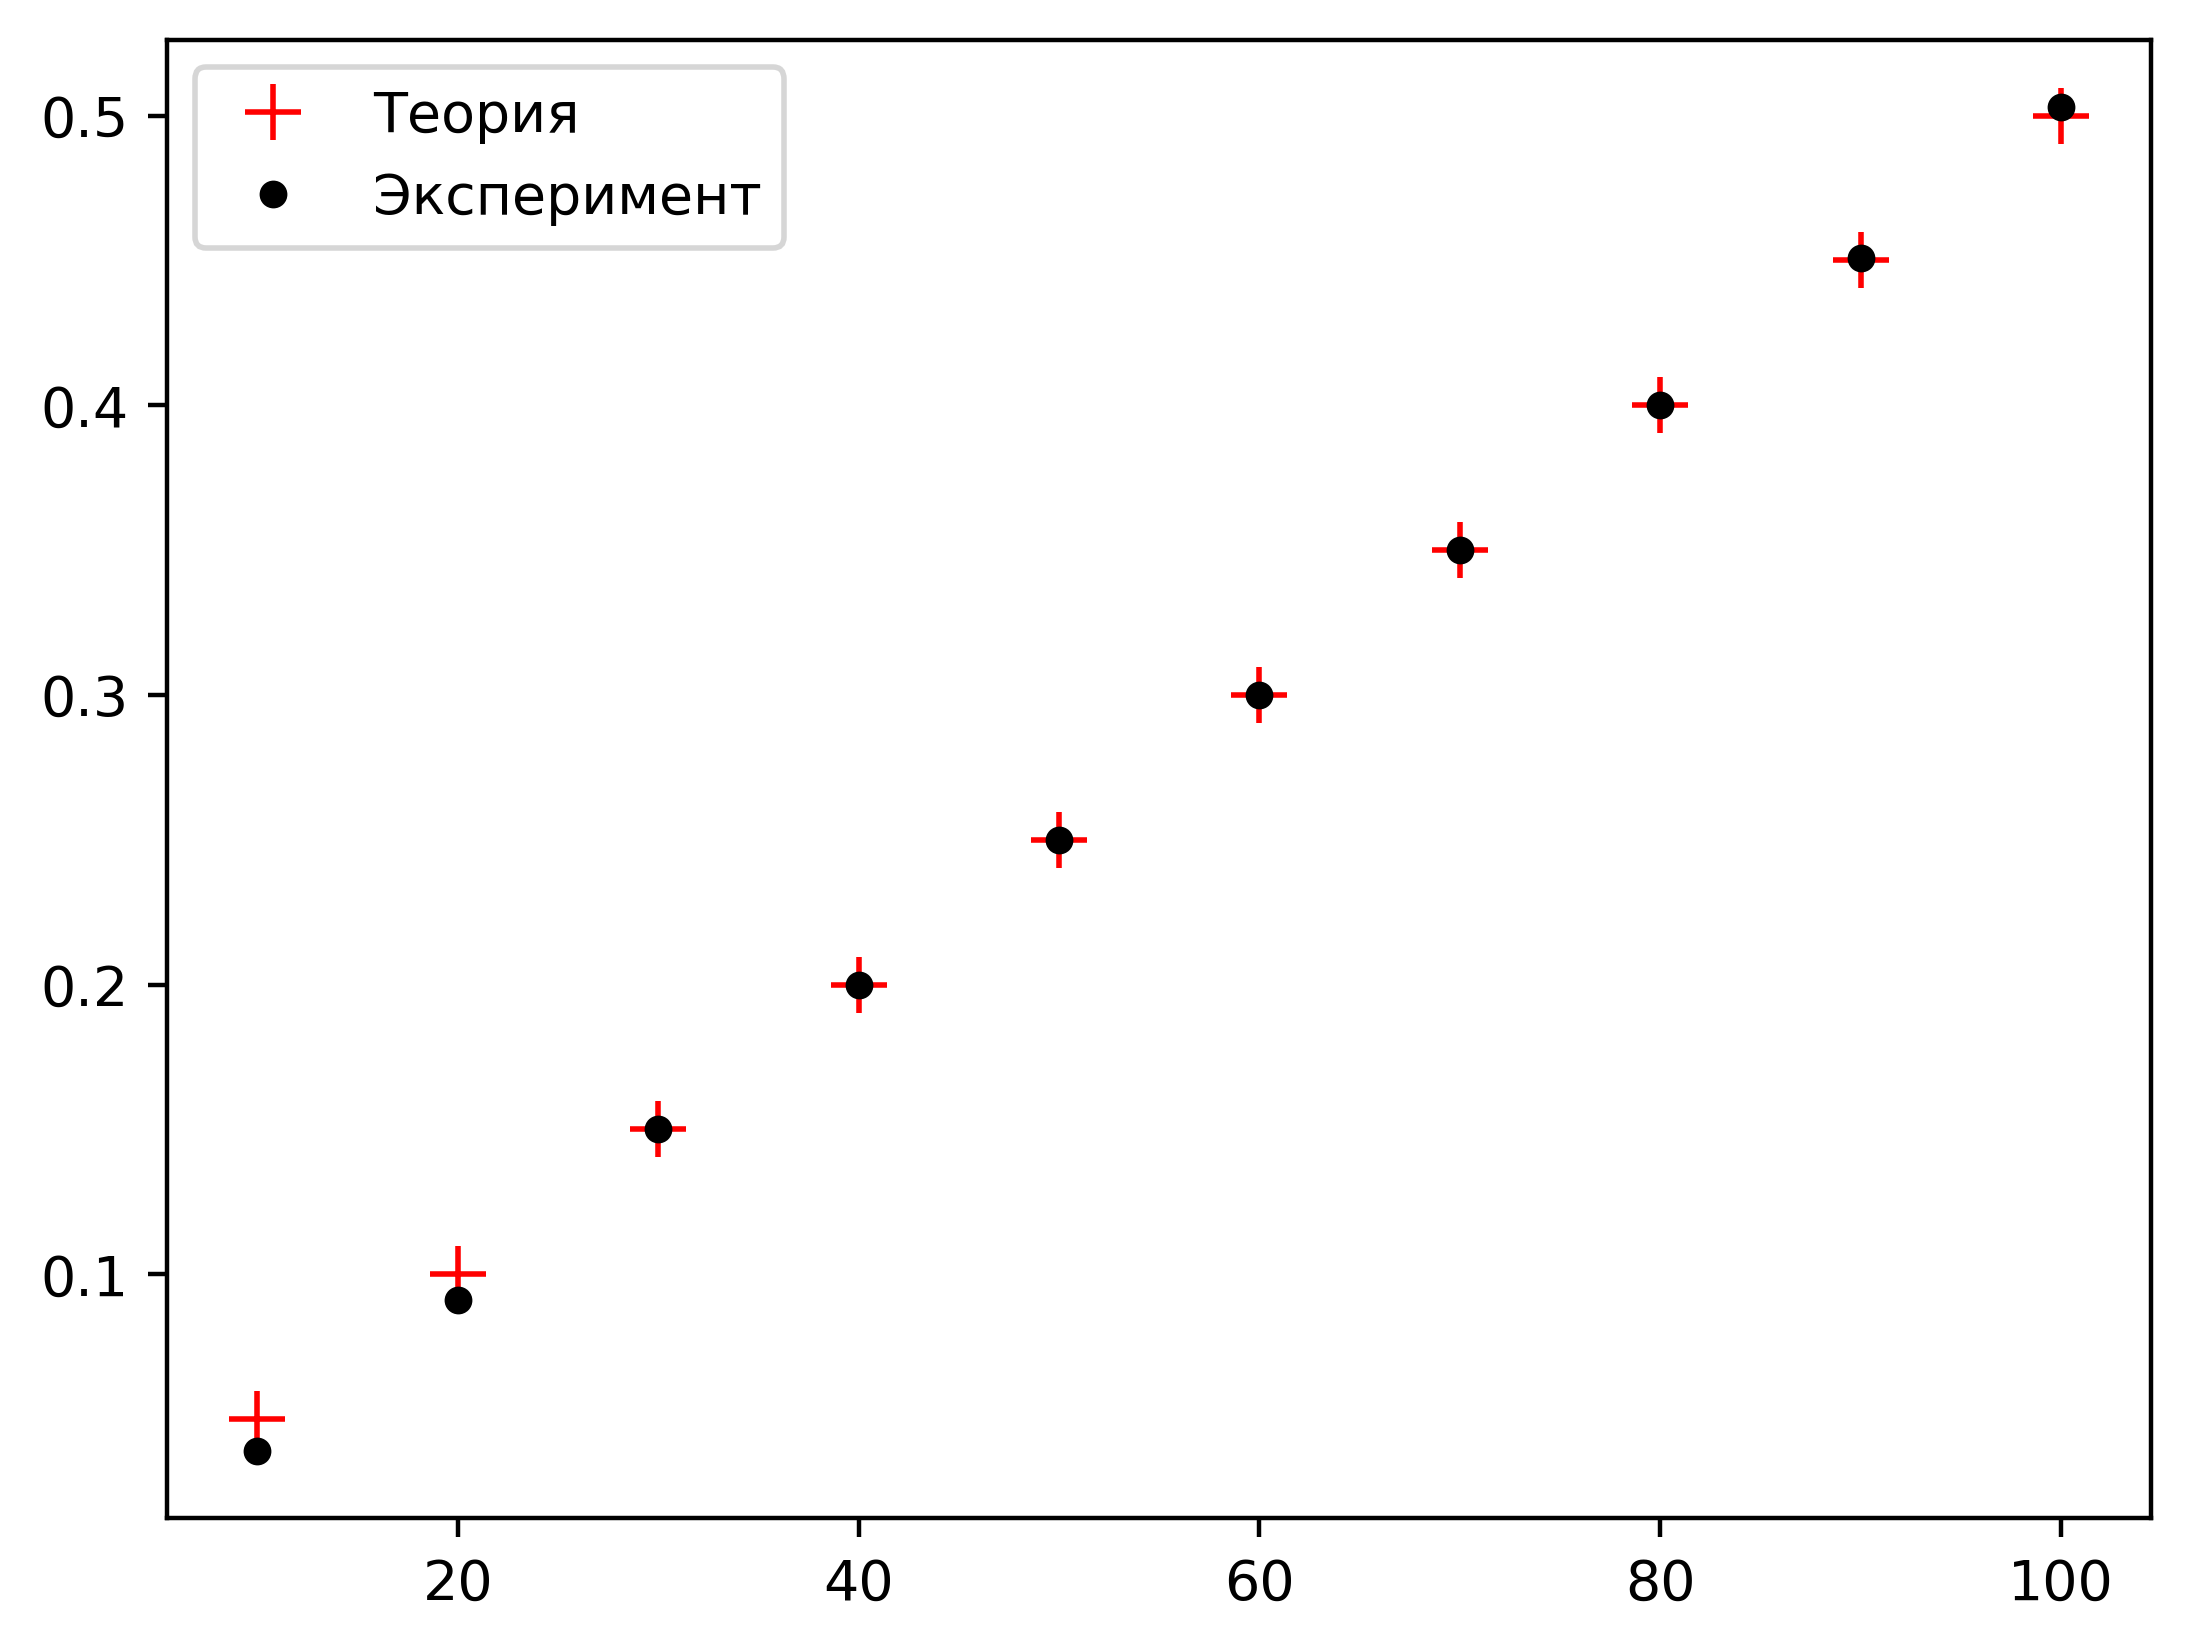
\includegraphics[width=0.6\linewidth]{pics/amplot}
  \caption{}
  \label{ammplot}
\end{figure}
Видно, что за искллючением критических значений ($\eta \sim 0\%, \eta \sim 100 \%$) практический результат хорошо сходится с теоретическим.

\subsection{Часть F. Изучение фильтрации сигналов}
Подадим на RC-фильтр последовательность прямоугольных импульсов, с базовым уровнем 0V. Картина отклика представлена на рис. \ref{RC}:
\begin{figure}[H]
  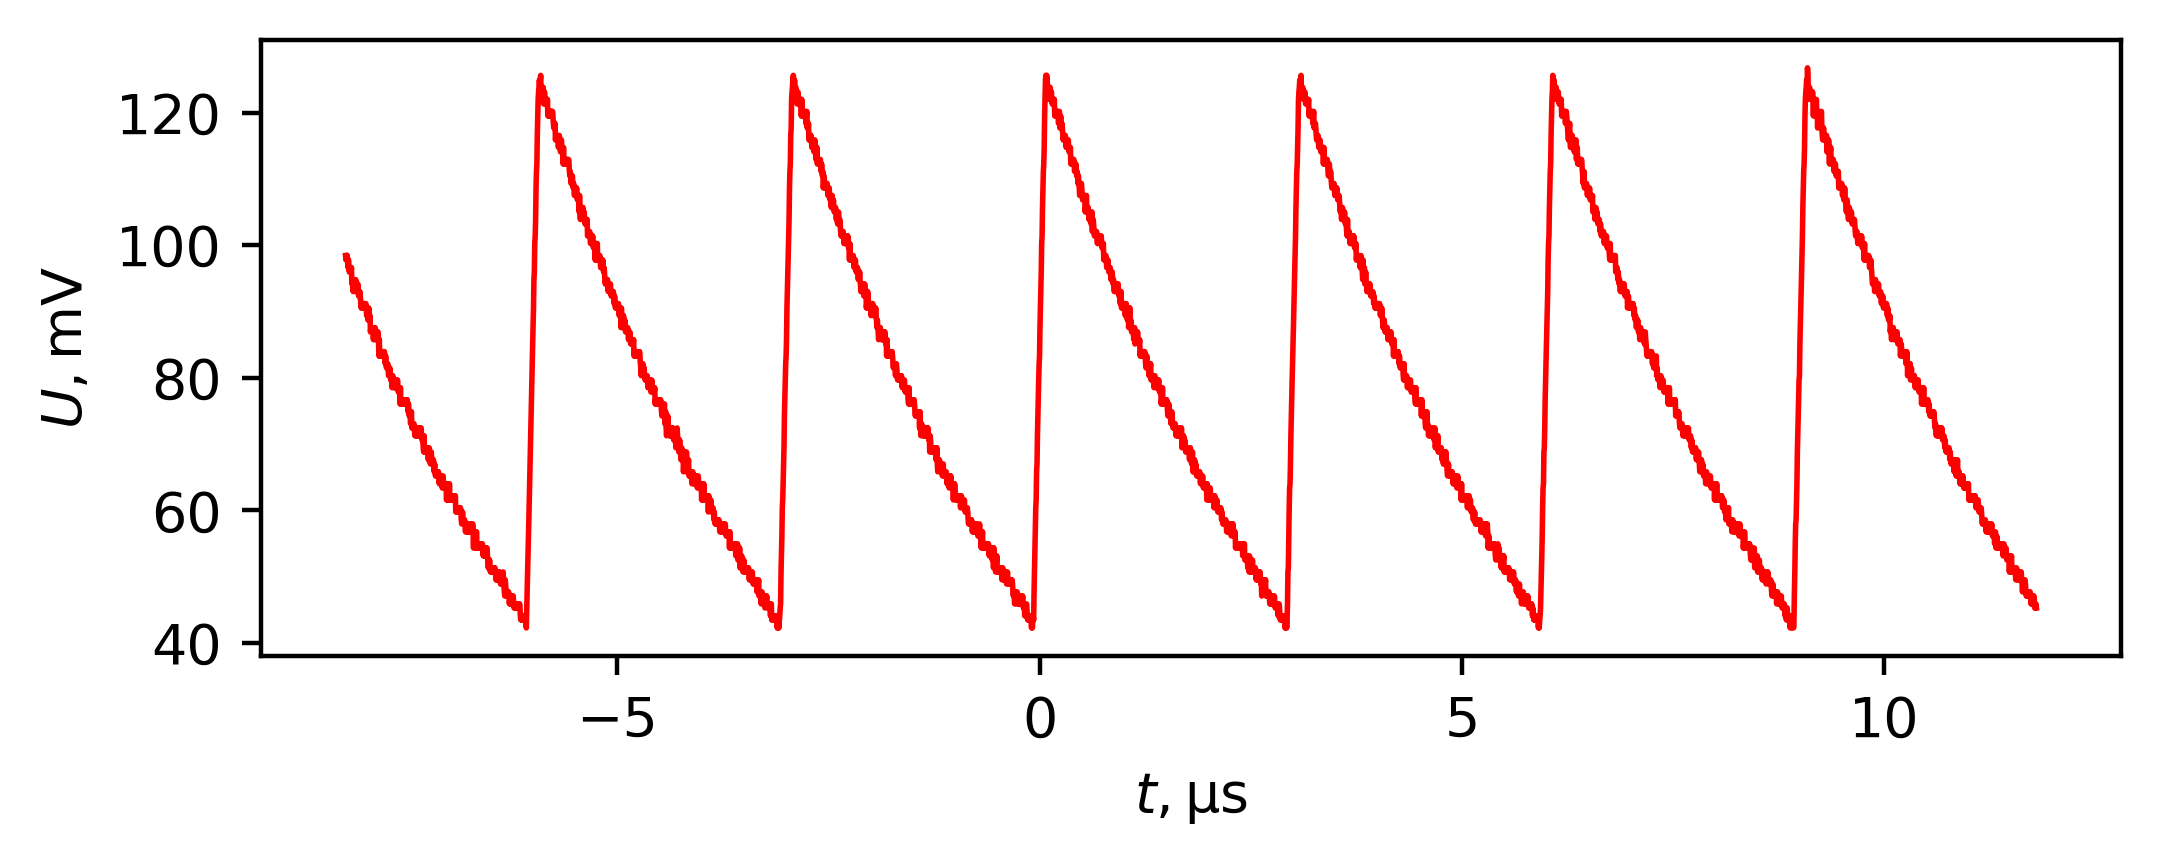
\includegraphics[width=0.8\linewidth]{pics/RC}
  \caption{Картина сигнала после фильтрации}
  \label{RC}
\end{figure}

Рассмотрим спектры исходного и обработанного сигналов:
\begin{figure}[H]
  \centering
  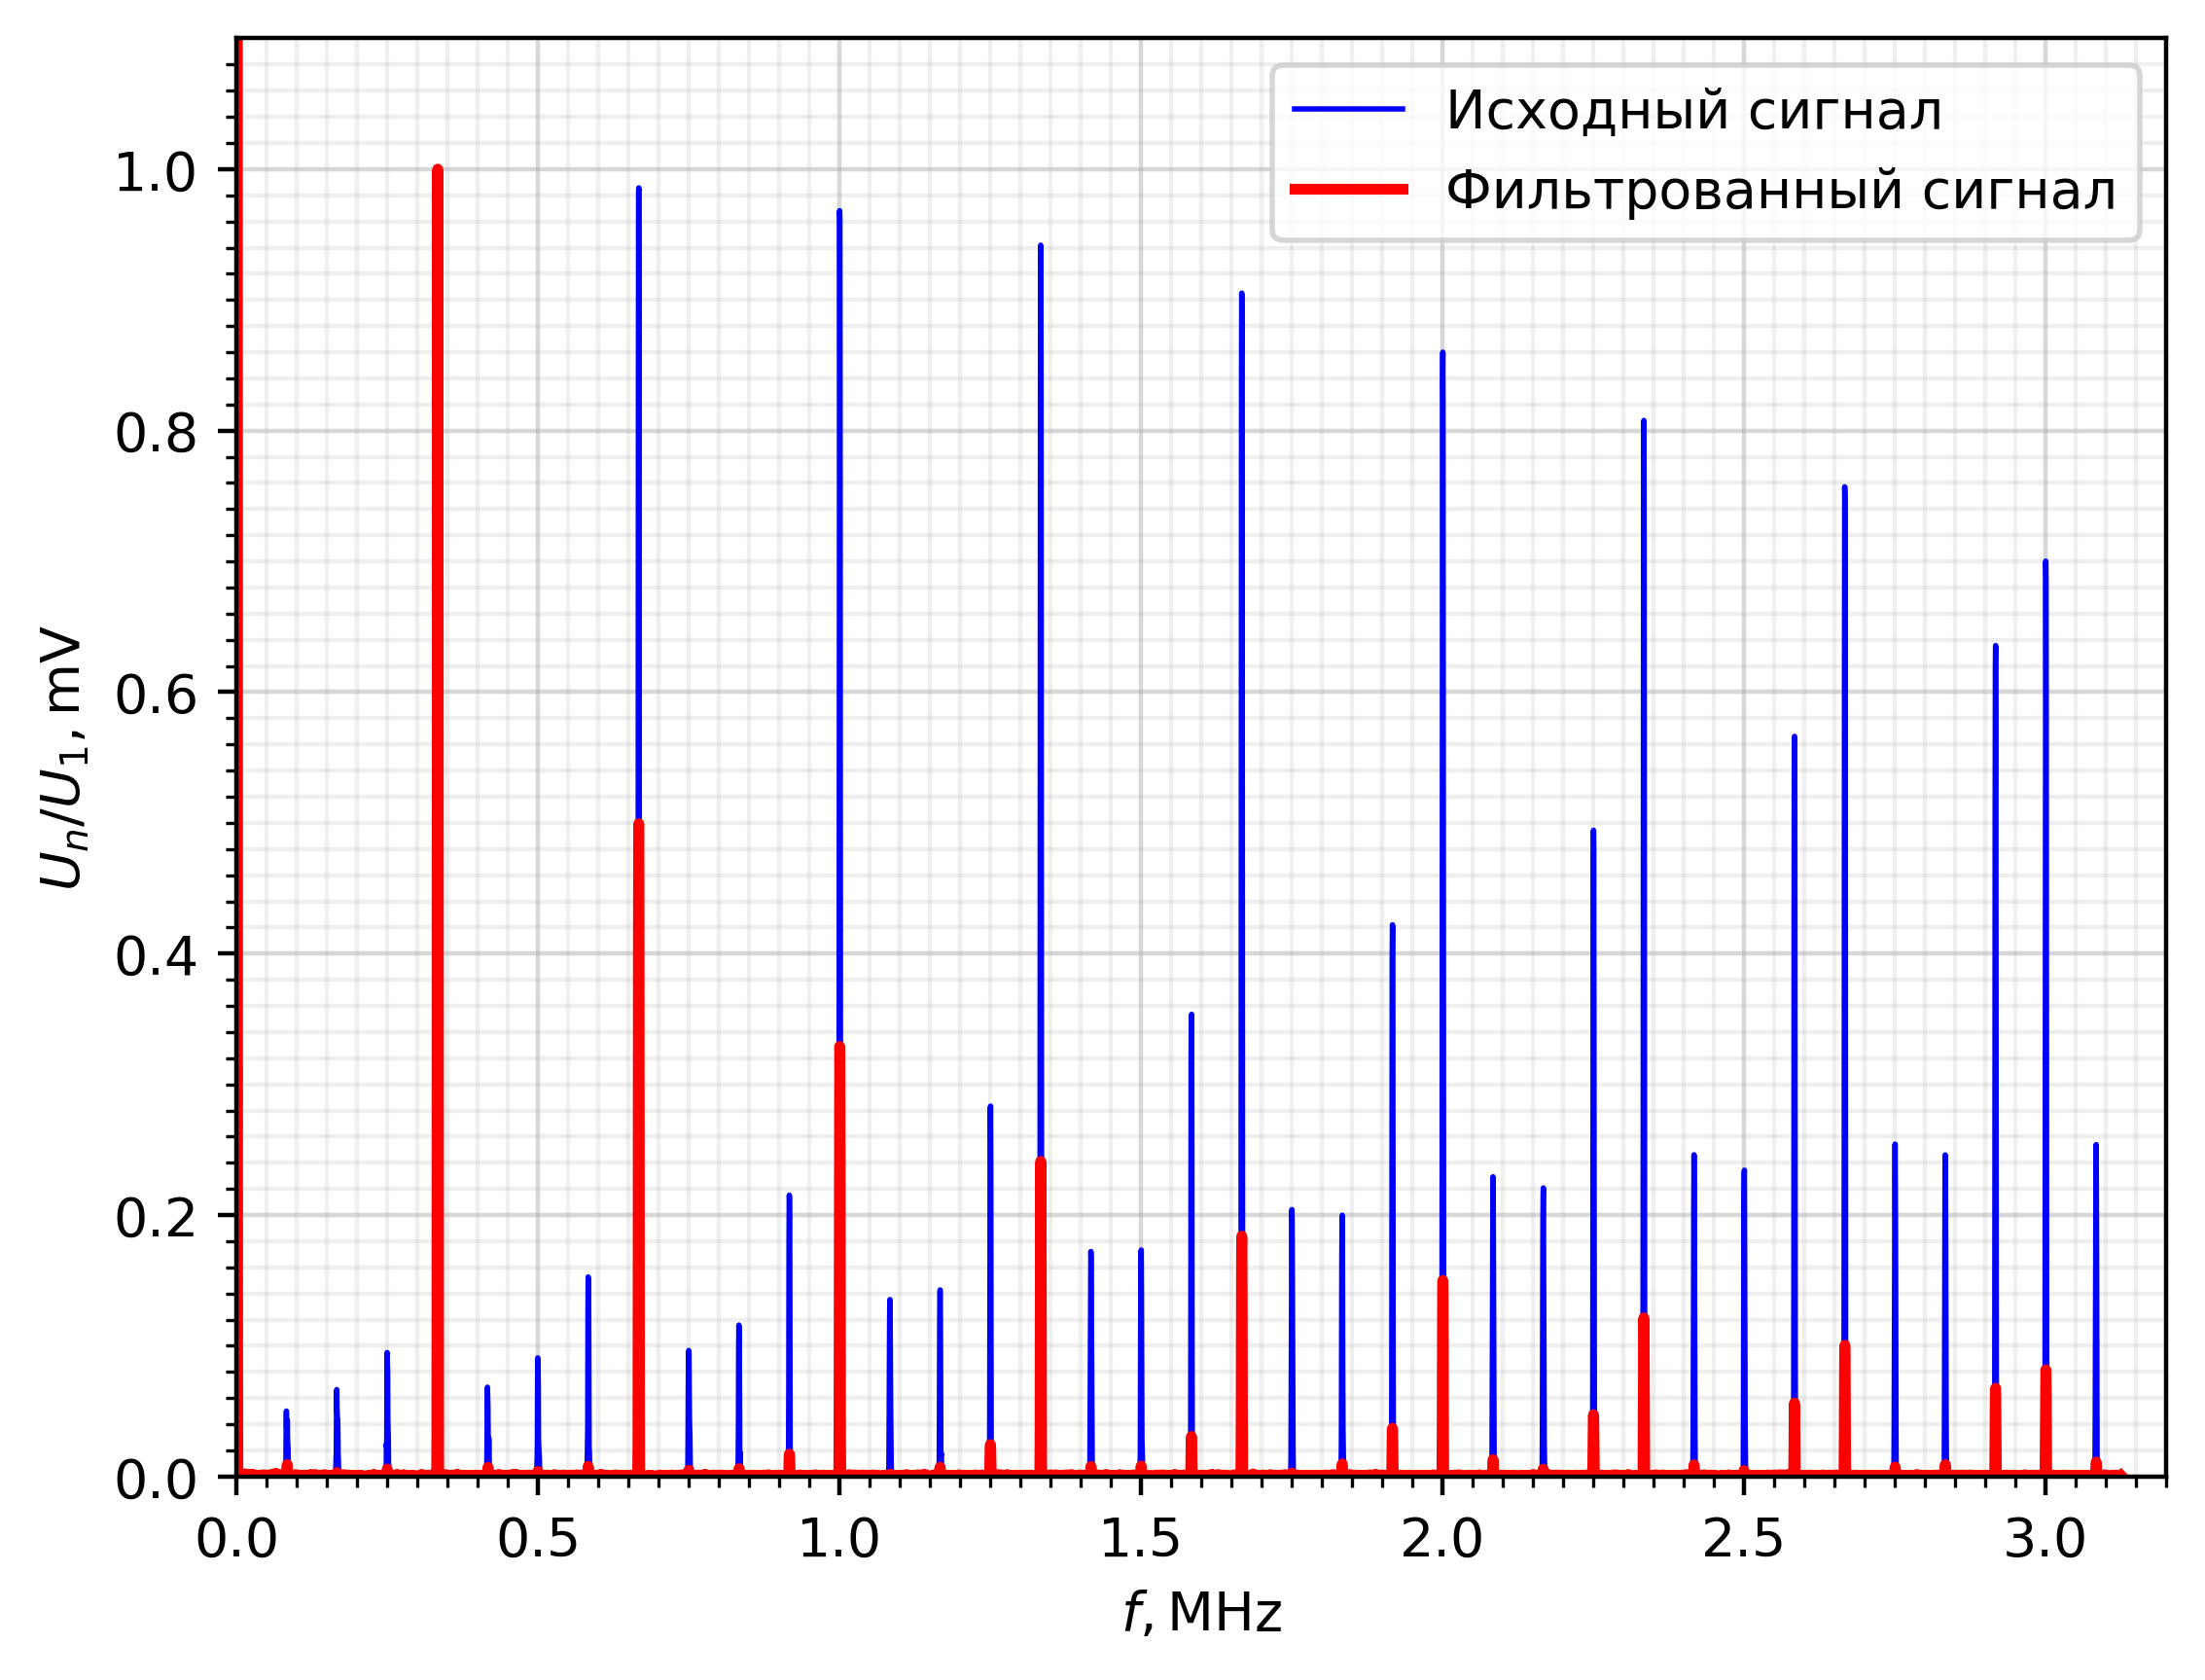
\includegraphics[width=0.8\linewidth]{pics/RCspec}
  \caption{Сравнение спектров исходного и отфильтрованного сигналов}
  \label{amplot}
\end{figure}

\section{Обсуждение результатов и выводы}
В ходе работы было снято достаточно много высококачественных спектров периодических сигналов разной формы (меандр, цуги, АМ), получена передаточная характеристика дифференцирующей RC-цепочки. Показана простота сравнения спектров подобных сигналов с различными параметрами с помощью соотношений неопределённости. Полученные спектры хорошо совпали с теоретическими ожиданиями.


\end{document}
